\documentclass[border=3pt]{standalone}
% Preâmbulo compartilhado pelos diagramas TikZ da aula 5 de IHC (Processos de Design)
\usepackage[T1]{fontenc}
\usepackage[utf8]{inputenc}
\usepackage{lmodern}
\usepackage{amsmath}
\usepackage{xcolor}
\usepackage{tikz}
\usetikzlibrary{arrows.meta,angles,quotes,decorations.pathmorphing,calc,
                positioning,shapes.geometric,shapes.misc,backgrounds,fit,
                math}

% Paleta (mesma dos SVGs originais)
% Paleta da disciplina de IHC: acento roxo (#755099), da capa do livro.
% (o nome "dblue" é mantido para não alterar todos os diagramas)
\definecolor{dblue}{HTML}{755099}
\definecolor{dorange}{HTML}{B3541E}
\definecolor{dgreen}{HTML}{4A7C59}
\definecolor{dred}{HTML}{9C4B4B}
\definecolor{dcream}{HTML}{F4F1EA}
\definecolor{dshade}{HTML}{DDD7C9}

% Função gaussiana (não normalizada por padrão de escala visual)
\pgfmathdeclarefunction{gauss}{3}{%
  \pgfmathparse{1/(#3*sqrt(2*pi))*exp(-((#1-#2)^2)/(2*#3^2))}%
}

% Estilos comuns (prefixo d... para não colidir com chaves internas do pgf)
\tikzset{
  >={Stealth[length=2mm]},
  dguide/.style={gray!55, dashed, line width=0.4pt},
  daxis/.style={gray!60, line width=0.7pt, ->},
  dbody/.style={fill=black!3, draw=black!80, line width=1pt},
  dacc/.style={draw=dblue, line width=1pt},
  dlbl/.style={black!55, font=\small},
  dsub/.style={black!45, font=\footnotesize},
  dstate/.style={circle, draw=black!80, fill=dcream, line width=1pt,
                 minimum size=17mm, font=\large, inner sep=1pt},
  dobs/.style={circle, draw=black!80, fill=dshade, line width=1pt,
               minimum size=14mm, font=\large, inner sep=1pt},
  dbox/.style={rounded corners=2pt, draw=black!80, fill=dcream, line width=1pt,
               align=center, inner sep=6pt},
  dop/.style={circle, draw=black!80, fill=white, line width=1pt,
              minimum size=6mm, inner sep=0pt, font=\small},
  dtrans/.style={->, dblue, line width=1pt},
  dmeas/.style={->, dorange, line width=1pt},
  dcurve/.style={line width=1pt, dblue},
  dcurveb/.style={line width=1.4pt, dorange},
}

\begin{document}
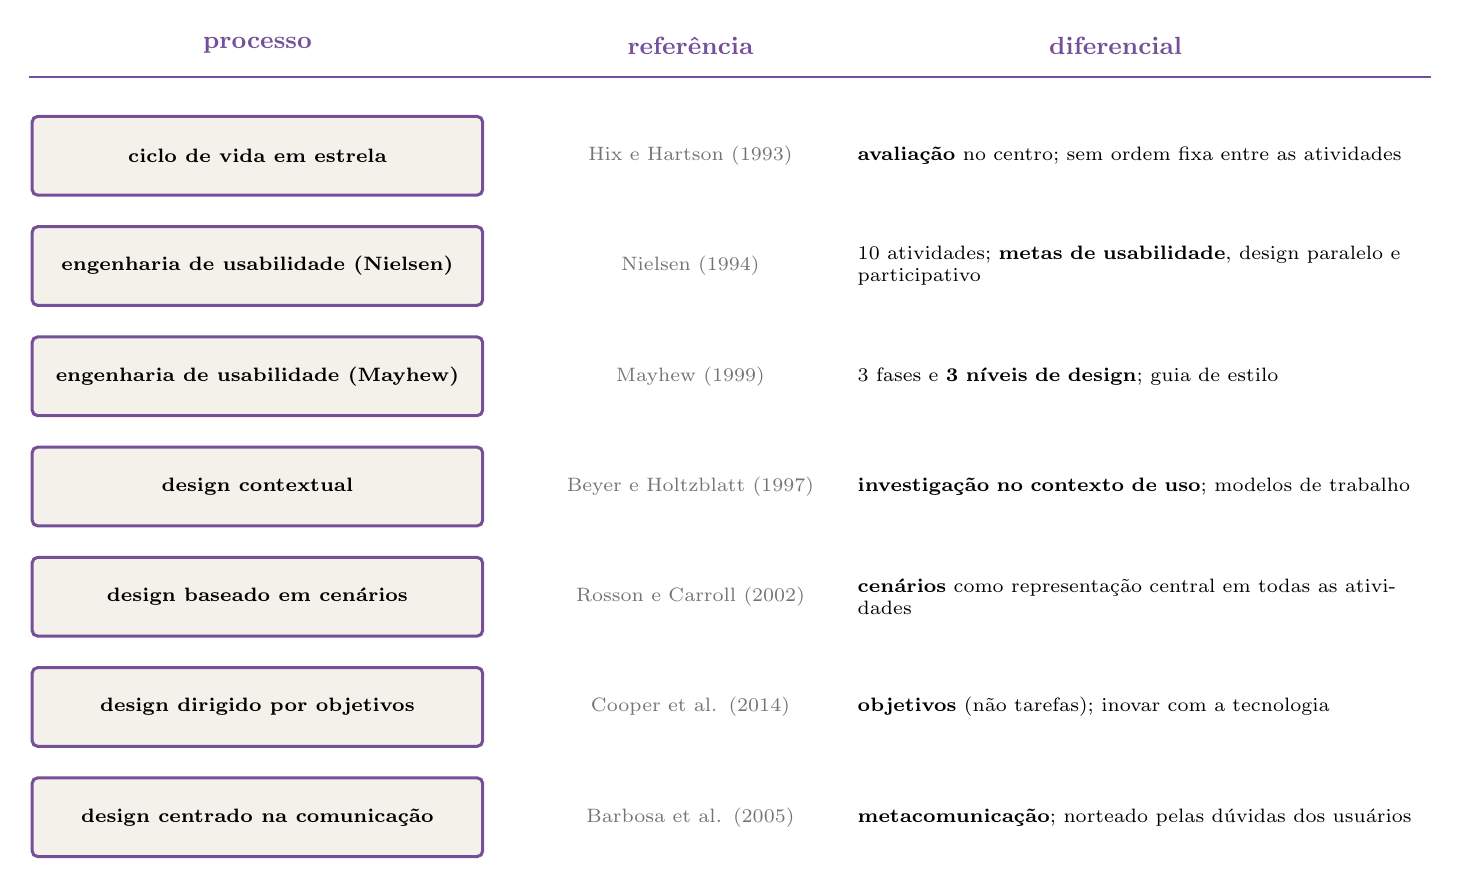
\begin{tikzpicture}[x=1cm,y=1cm,
   nm/.style={dbox, text width=5.3cm, minimum height=1.0cm, font=\scriptsize\bfseries, draw=dblue, line width=1.1pt},
   rf/.style={font=\scriptsize, text width=3.4cm, align=center, text=black!55},
   df/.style={font=\scriptsize, text width=7.4cm, align=left}]

  \node[font=\small\bfseries, dblue] at (2.7,0.9) {processo};
  \node[font=\small\bfseries, dblue] at (8.2,0.9) {referência};
  \node[font=\small\bfseries, dblue] at (13.6,0.9) {diferencial};
  \draw[dblue, line width=1pt] (-0.2,0.5) -- (17.6,0.5);

  \node[nm] at (2.7,-0.5) {ciclo de vida em estrela};
  \node[rf] at (8.2,-0.5) {Hix e Hartson (1993)};
  \node[df, anchor=west] at (10.2,-0.5) {\textbf{avaliação} no centro; sem ordem fixa entre as atividades};

  \node[nm] at (2.7,-1.9) {engenharia de usabilidade (Nielsen)};
  \node[rf] at (8.2,-1.9) {Nielsen (1994)};
  \node[df, anchor=west] at (10.2,-1.9) {10 atividades; \textbf{metas de usabilidade}, design paralelo e participativo};

  \node[nm] at (2.7,-3.3) {engenharia de usabilidade (Mayhew)};
  \node[rf] at (8.2,-3.3) {Mayhew (1999)};
  \node[df, anchor=west] at (10.2,-3.3) {3 fases e \textbf{3 níveis de design}; guia de estilo};

  \node[nm] at (2.7,-4.7) {design contextual};
  \node[rf] at (8.2,-4.7) {Beyer e Holtzblatt (1997)};
  \node[df, anchor=west] at (10.2,-4.7) {\textbf{investigação no contexto de uso}; modelos de trabalho};

  \node[nm] at (2.7,-6.1) {design baseado em cenários};
  \node[rf] at (8.2,-6.1) {Rosson e Carroll (2002)};
  \node[df, anchor=west] at (10.2,-6.1) {\textbf{cenários} como representação central em todas as atividades};

  \node[nm] at (2.7,-7.5) {design dirigido por objetivos};
  \node[rf] at (8.2,-7.5) {Cooper et al. (2014)};
  \node[df, anchor=west] at (10.2,-7.5) {\textbf{objetivos} (não tarefas); inovar com a tecnologia};

  \node[nm] at (2.7,-8.9) {design centrado na comunicação};
  \node[rf] at (8.2,-8.9) {Barbosa et al. (2005)};
  \node[df, anchor=west] at (10.2,-8.9) {\textbf{metacomunicação}; norteado pelas dúvidas dos usuários};

\end{tikzpicture}
\end{document}
